\section{IPC}
\acrfull{ipc} predstavuje súbor mechanizmov určených na komunikáciu a správu dát medzi viacerými procesmi. Operačný systém Linux obsahuje niekoľko takýchto mechanizmov, medzi najhlavnejšie patria:
\begin{itemize}
\item Signály
\item Rúry
\item Fronty správ
\item Semafory
\item Zdieľaná pamäť
\item Sokety
\end{itemize}
Jadro operačného systému Linux obsahuje dve rôzne implementácie pre semafory, fronty správ a zdieľanú pamäť. Tieto implementácie sa nazývajú \textit{System V} a \textit{POSIX}. \textit{System V} je staršia implementácia, ktorá je odvodená od komerčného Unix systému \textit{System V}. Implementácia \textit{POSIX} je štandard, ktorý taktiež implementuje tieto mechanizmy avšak funkcie a systémové volania sa líšia. Každá implementácia má svoje výhody a nevýhody, avšak implementácia \textit{POSIX} bola vyvinutá neskôr ako \acrshort{lsm} a teda nemá vytvorené \acrshort{lsm} \textit{hooky}, ktoré by mali dopad na túto diplomovú prácu. Preto v nasledujúcich odsekoch budeme popisovať \textit{System V} semafory(ďalej len semafory), \textit{System V} fronty správ(ďalej len fronty správ) a \textit{System V} zdieľanú pamäť(ďalej len zdieľaná pamäť).
\subsection{Signály}
Ide o jeden z najstarších \acrshort{ipc} mechanizmov používaný v Unix systémoch. Signál je asynchrónne upozornenie zaslané procesu alebo konkrétnemu vláknu v rámci toho istého procesu, za účelom upozornenia na udalosť, ktorá sa vyskytla. V momente keď sa signál odošle, operačný systém preruší vykonávanie procesu, ktorý má byť signalizovaný a v tomto procese sa vykoná obslúženie signálu.\cite{signal}

Je potrebné si uvedomiť že \textbf{signály nie sú} to isté ako \textbf{prerušenia}. Rozdiel medzi signálom a prerušením je, že prerušenie je vyvolané procesorom a signál je vyvolaný z jadra systému.
Signál je možné vyvolať systémovým volaním \textbf{kill}. Toto systémové volanie má dva parametre\cite{kill}:
\begin{itemize}
\item \textit{pid} - identifikátor procesu, ktorý má byť signalizovaný
\item \textit{sig} - typ signálu
\end{itemize}
Podporované typy je možné zistiť pomocou príkazu \textit{kill -l} alebo v súbore \textit{/include/linux/signal.h}.

V prípade že je definovaná obslužná funkcia, táto funkcia sa vykoná, v opačnom prípade je použitá štandardná obsluha signálu. Obslužnú funkciu je možné definovať pomocou funkcie \textbf{signal}, avšak správanie tejto funkcie môže byť rozdielne vzhľadom na platformu. Preto sa odporúča používať funkciu \textbf{sigaction}, ktorá bola definovaná v štandarde \textbf{POSIX.1}. Toto systémové volanie má parametere\cite{sigaction}:
\begin{itemize}
\item \textit{signum} - typ signálu, ktorý chceme obslúžiť
\item \textit{act} - definuje akciu, ktorá sa má vykonať pri obsluhe signálu
\item \textit{oldact} - definuje starú obsluhu signálu
\end{itemize}

\textbf{Signály} je možné použiť pre komunikáciu ako aj synchronizáciu avšak ide o veľmi slabý nástroj pre tieto potreby.\footnote{\url{http://man7.org/conf/lca2013/IPC_Overview-LCA-2013-printable.pdf}}
\subsection{Rúry}
Rúry predstavujú jednosmerný tok dát medzi procesmi: všetky dáta zapísané procesom do rúry sú jadrom   presmerované do iného procesu, ktorý z nej môže čítať. Poznáme 2 druhy rúr \cite{linux}:
\begin{itemize}
\item Anonymné rúry - žiadny objekt v súborovom strome
\item Pomenované rúry - objekt v súborovom strome
\end{itemize}
\subsubsection{Anonymné rúry}
\textbf{Anonymné rúry} je možné vytvoriť pomocou systémového volania \textbf{pipe}, alebo taktiež pomocou znaku \textbf{|} vo väčšine \textit{Unix} príkazových riadkoch.Systémové volanie \textbf{pipe} obsahuje jeden parameter, ktorým je pole \textit{pipefd} o veľkosti 2. Toto pole obsahuje po návrate z funkcie súborové deskriptory. Tieto dva súborové deskriptory predstavujú konce rúry, \textit{pipefd[0]} je čítací koniec rúry a \textit{pipefd[1]} je zapisovací koniec rúry. Tieto súborové deskriptory je následne možné použiť na zapisovanie a čítanie pomocou systémových volaní \textit{write}\footnote{\url{http://man7.org/linux/man-pages/man2/write.2.html}} a \textit{read}\footnote{\url{http://man7.org/linux/man-pages/man2/read.2.html}}. Tieto operácie sú blokujúce v dvoch prípadoch:
\begin{itemize}
\item write - rúra je plná
\item read - rúra je prázdna
\end{itemize}
Niektoré \textit{Unix} systémy ako napríklad \textit{System V Release 4}, implementuje \textbf{full-duplex} rúry, teda rúry, pri ktorých oba konce rúry(súborové deskriptory) je možné použiť ako na zapisovanie tak aj na čítanie. Avšak štandard \textbf{\acrshort{posix}} definuje iba \textbf{half-duplex} rúry, pričom každý proces musí zatvoriť jeden deskriptor pred použitím druhého.\cite{linux}

Takto vytvorená rúra umožňuje komunikáciu medzi rodičovským procesom a jeho potomkami. Avšak je potrebné zabezpečiť aby procesy, ktoré medzi sebou chcú komunikovať zdieľali rovnaké súborové deskriptory. Toto je možné jednoducho dosiahnuť tak, že sa rúra vytvorí pred vytvorením detského procesu(\textit{fork}). Zjednodušený pseudokód môžeme vidieť na ukážke kódu \ref{lst:pipe-c} spolu s ilustračný obrázkom \ref{pipeflow}.\cite{overview}
\begin{lstlisting}[
  caption={Použite anonymných rúr},
  label={lst:pipe-c},
  language=c
]
int filedes[2];

pipe(filedes);

child_pid = fork();
if (child_pid == 0) {
	close(filedes[1]);
} else {
	close(filedes[1]);
}
\end{lstlisting}
\begin{figure}[!htbp]
  \centering
  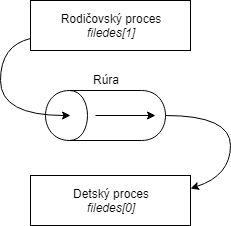
\includegraphics[width=5cm]{img/rura.png}
  \caption{Tok dát medzi procesmi.}
  \label{pipeflow}
\end{figure}

Nevýhodou tohto systémového volania je absencia v súborovom strome a teda nie je možné využiť tento \acrshort{ipc} mechanizmus na komunikáciu medzi ľubovoľnými dvoma alebo viacerými procesmi.\cite{overview}
\subsubsection{Pomenované rúry}
Pomenované rúry taktiež nazývané aj \textbf{\acrshort{fifo}} na rozdiel od anonymných rúr máju meno v súborovom systéme. Jednou z možností ako vytvoriť tento typ rúry je pomocou funkcie \textbf{mkfifo}, ktorá je definovaná v štandarde \acrshort{posix}. Táto funkcia v svojej implementácií volá systémové volanie \textit{mknod} s príznakom, ktorý definuje že ide o pomenovanú rúru. Funkcia \textbf{mkfifo} má 2 parametre:
\begin{itemize}
\item \textit{pathname} - názov rúry
\item \textit{mode} - práva súboru 
\end{itemize}
Návratová hodnota funkcie je 0 v prípade úspechu a v prípade chyby je návratová hodnota -1. Takto vytvorenú rúru je možné rovnako ako anonymné rúry obsluhovať pomocou systémových volaní \textit{read} a \textit{write}.\cite{mkfifo}

\subsection{Fronty správ}
Fronty správ si najlepšie môžme predstaviť ako zreťazený zoznam v adresnom priestore jadra. Správy môžu byť odosielané do fronty v poradí a následne načítané z fronty pomocou niekoľko rôznych spôsobov. Každá fronta správ je jednoznačne identifikovaná pomocou \acrshort{ipc} identifikátora. Pre lepšie pochopenie tohto konceptu si popíšeme 3 hlavné štruktúry, ktoré zabezpečujú fungovanie fronty správ v jadre Linuxu.\cite{guide}
\subsubsection{Štruktúry fronty správ} \label{msgstruct}
Štruktúra \texttt{msgbuf} (definovaná v \url{linux/msg.h}) predstavuje predlohu ako by mala vyzerať správa, ktorú budeme posielať. Táto predloha obsahuje dve položky: 
\begin{itemize}
\item long \textbf{mtype} - umožňuje určiť o aký typ správy ide, napríklad \textit{chybová správa}, \textit{normálna správa} a podobne, možností je nekonečno
\item char \textbf{mtext}[1] - samotné dáta správy, túto položku je možné ľubovoľne rozšíriť, ako napríklad na ukážke kódu \ref{lst:msgbuf}, avšak s limitom, ktorý je maximálna dĺžka správy \textit{\textbf{MSGMAX}}=8192\footnote{Táto veľkosť je definovaná v \url{linux/msg.h} a môže sa líšiť od verzie jadra. Túto hodnotu je taktiež možné zistiť pomocou príkazu \textit{ipcs -l}.}
\end{itemize}

\begin{lstlisting}[
  caption={Príklad vlastnej štruktúry správy},
  label={lst:msgbuf},
  language=c
]
struct message {
    long type;
    struct my_special_struct data;    
} msg;
\end{lstlisting}

Každá správa je rozdelená na stránky, ktoré sú dynamicky alokované v pamäti. Veľkosť tejto stránky je závislí od architektúry a zisťuje sa nasledovne \textit{sysconf(\_SC\_PAGESIZE)}. Štruktúra \textbf{\textit{msg\_msg}}, ktorú môžeme vidieť na výpise štruktúry \ref{lst:msgmsg}, predstavuje hlavičku každej správy pričom sa inštancie tejto štruktúry nachádzajú v zreťazenom zozname, ktorý je definovaný položkou \textit{m\_list}. V prípade že dĺžka správy je menšia ako $$ \text{PAGE\_SIZE} - \text{sizeof(struct msg\_msg)} $$ celý obsah správy sa nachádza v pamäťovej oblasti za štruktúrou \textit{msg\_msg}. V opačnom prípade sa prvá časť správy nachádza na rovnakom mieste a ostatné stránky sa nachádzajú v pamäťovej oblasti, na ktorú ukazuje ukazovateľ \textit{next}. Tento ukazovateľ odkazuje na štruktúru \textit{msg\_msgseg}, ktorej položky môžeme vidieť na definícii štruktúry \ref{lst:msgmsgseg}, ktorá obsahuje ukazovateľ \textit{next} na ďalšiu stránku, pričom v pamäťovej oblasti za touto štruktúrou sa nachádzajú dáta aktuálnej stránky.
\begin{lstlisting}[
  caption={Štruktúra msg\_msg},
  label={lst:msgmsg},
  language=c
]
struct msg_msg {
	struct list_head m_list;
	long m_type;
	size_t m_ts;
	struct msg_msgseg *next;
	void *security;
	/* obsah prvej stránky */
};
\end{lstlisting}

\begin{lstlisting}[
  caption={Štruktúra msg\_msgseg},
  label={lst:msgmsgseg},
  language=c
]
struct msg_msgseg {
	struct msg_msgseg *next;
	/* obsah stránky */
};
\end{lstlisting}

Poslednou štruktúrou, ktorá sa nachádza najvyššie v hierarchií týchto štruktúr je \texttt{\textbf{msq\_queue}} a jej deklaráciu môžete vidieť na ukážke kódu \ref{lst:msgmsgseg}. Najdôležitejšou položkou tejto štruktúry je položka\texttt{q\_messages}, ktorá predstavuje prvý element zreťazeného zoznamu všetkých správ vo fronte. Ďalšie zreťazené zoznamy, ktoré sa tu nachádzajú sú \texttt{q\_receivers} a \texttt{q\_senders}, ktoré obsahujú zreťazené zoznamy procesov, ktoré posielajú správy a procesov, ktoré prijímajú správy. Zaujímavou položkou z pohľadu bezpečnosti je položka \texttt{q\_perm}, ktorá obsahuje inštanciu štruktúry \texttt{\textbf{kern\_ipc\_perm}}. Túto štruktúru si popíšeme v kapitole \ref{kernipcperm}.\cite{linux}
\begin{lstlisting}[
  caption={Štruktúra msq\_queue},
  label={lst:msgmsgseg},
  language=c
]
struct msg_queue {
	struct kern_ipc_perm q_perm;
	/* meta dáta */		
	struct list_head q_messages;
	struct list_head q_receivers;
	struct list_head q_senders;
} __randomize_layout;
\end{lstlisting}
\subsubsection{Štruktúra kern\_ipc\_perm} \label{kernipcperm}
Štruktúra \texttt{kern\_ipc\_perm} sa nenachádza len pri fronte správ ale taktiež aj pri semaforoch a zdieľanej pamäti. Táto štruktúra predstavuje sadu meta dát o konkrétnom \acrshort{ipc} objekte a jej položky spolu s typmi môžeme vidieť na ukážke kódu \ref{lst:kernipcperm}. Vyznám týchto položiek je nasledovný:
\begin{itemize}
\item lock - uzamykací mechanizmus pre ochranu \acrshort{ipc} objektu
\item deleted - príznak, či bol zdroj uvoľnený
\item id
\item key - jednoznačný identifikátor, v rámci konkrétneho typu objektu, to znamená, že jedna inštancia semafora, zdieľanej pamäte alebo fronty správ môže mať rovnaký identifikátor
\item uid - ID používateľa, ktorý vlastní \acrshort{ipc} objekt
\item gid - ID skupiny, ktorá vlastní \acrshort{ipc} objekt
\item cuid - ID používateľa, ktorý vytvoril \acrshort{ipc} objekt
\item cgid - ID skupiny, ktorá vytvorila \acrshort{ipc} objekt
\item mode - bitová maska oprávnení
\item seq - sekvenčné číslo, používané sa na vytvorenie nového identifikátora pre \acrshort{ipc} objekt
\item security - ukazovateľ na štruktúru, ktorú vytvára zvolené bezpečnostné riešenie v jadre Linuxu
\item khtnode
\item rcu - \acrshort{rcu} synchronizačný mechanizmus
\item refcount - počítadlo použití \acrshort{ipc} objektu
\end{itemize}
\subsubsection{Požívanie fronty správ} \label{msguse}
Na vytvorenie fronty správ sa používa systémové volanie \texttt{msgget}. Toto systémové volanie má dva parametre, ktorými sú \texttt{key}(identifikátor objektu) a \texttt{msgflg} príznaky \acrshort{ipc} objektu. Nová fronta je vytvorená v prípadoch, že:
\begin{itemize}
\item \texttt{key} sa rovná \texttt{IPC\_PRIVATE}
\item \texttt{key} nemá ešte priradený žiadny \acrshort{ipc} objekt a \texttt{IPC\_CREATE} príznak je definovaný v parametre \texttt{msglfg}
\end{itemize}
Ak je definovaný príznak \texttt{IPC\_EXCL} spolu s \texttt{IPC\_CREATE} a identifikátor už existuje, volanie funkcie zlyhá s chybovou správou \texttt{EEXIST}, ktorá definuje, že \acrshort{ipc} objekt už existuje. Naopak v prípade, že \texttt{IPC\_EXCL} nie je definované tak návratová hodnota je identifikátor už existujúceho \acrshort{ipc} objektu.\cite{msgget}

Na posielanie a prijímanie správ z fronty sa používajú systémové volania \texttt{msgsnd} a \texttt{msgrcv}. Funkcia \texttt{msgsnd} má nasledovné parametre\cite{msgop}:
\begin{itemize}
\item \texttt{msgid} identifikátor fronty získaný z funkcie \texttt{msgget}
\item \texttt{msgp} ukazovateľ na štruktúru, ktorú si používateľ definuje sám a mal by vychádzať zo šablóny ktorú sme si popísali v kapitole \ref{msgstruct}
\item \texttt{msgsz} veľkosť dátovej štruktúry, ktorú chceme prenášať
\item \texttt{msgflg} príznaky, ktoré definujú čo sa má diať v prípade, že je fronta plná
\end{itemize}
Funkcia \texttt{msgrcv}, odstráni správu z frontu a premiestni do pamäte, na ktorý ukazuje parameter funkcie \texttt{msgp}. Ďalšie parametre sú\cite{msgop}:
\begin{itemize}
\item \texttt{msgsz} maximálnu veľkosť dát v bytoch pre položku \texttt{mtext}, štruktúry, na ktorú ukazuje ukazovateľ \texttt{msgp}
\item \texttt{msgflg} príznaky, ktoré definujú čo sa má diať v prípade, že je fronta prázdna
\item \texttt{msgtyp} číslo, ktoré definuje ktorý typ správy bude ako prvý vybraný z fronty(nemôže byt definovaný príznak \texttt{MSG\_COPY}), v prípade že je definovaný príznak \texttt{MSG\_EXCEPT}, tak sa z fronty vyberá prvá správa z typom odlišným od \texttt{msgtyp}
\end{itemize}
Posledným systémovým volaním tohto mechanizmu je \texttt{msgctl}, ktoré vykonáva kontrolné operácie nad objektom. Funkcia má 3 parametre\cite{msgctl}:
\begin{itemize}
\item \texttt{msgid} identifikátor objektu
\item \texttt{cmd} typ operácie
\item \texttt{buf} ide o štruktúru, ktorá sa v jadre ako aj v manuálových stránkach nachádza v 32 bitovej verzií(viď \ref{lst:msqid}), avšak v jadre sa označuje za zastaralú pričom ju nahrádza 64 bitová verzia(viď \ref{lst:msqid64}), táto štruktúra slúži na prenos meta dát z jadra systému do užívateľského priestoru
\end{itemize}
Typy operácie nad frontami správ sú nasledovné\cite{msgctl}:
\begin{itemize}
\item \texttt{IPC\_STAT} a \texttt{MSG\_STAT} kopíruje informácie z jadra do štruktúry na ktorú ukazuje ukazovateľ \texttt{buf}
\item \texttt{IPC\_SET} nastavuje položky jadra na základe ukazovateľa \texttt{buf}, konkrétne \texttt{msg\_perm.uid}, \texttt{msg\_perm.gid}, \texttt{msg\_qbytes} a posledných 9 bitov \texttt{msg\_perm.mode}
\item \texttt{IPC\_RMID} odstraňuje frontu správ
\item \texttt{IPC\_INFO} a \texttt{MSG\_INFO} získava limity a systémové nastavenia pre fronty správ, dáta sa nachádzajú na adrese ukazovateľa \texttt{buf}, avšak dáta sú v štruktúre typu \texttt{msginfo}(viď \ref{lst:msginfo}) a preto je potrebné pre-typovanie\footnote{\texttt{IPC\_INFO} a \texttt{MSG\_INFO} ako aj \texttt{IPC\_STAT} a \texttt{MSG\_STAT} vracajú mierne odlišné dáta a sú platformovo závislé pre viac info pozri \url{http://man7.org/linux/man-pages/man2/msgctl.2.html}}
\end{itemize}
\subsection{Semafory}
Semafor ako \acrshort{ipc} mechanizmus nepredstavuje nástoj na prenášanie dát ale slúži ako synchronizačný mechanizmus na ochranu zdieľaných zdrojov pri viac procesovom alebo viac vláknovom vykonávaný programu. Všeobecný semafor si môžme predstaviť ako počítadlo, ktoré je možné atomický upravovať. Semafor zvyčajne implementuje dve základné funkcie, ktoré slúžia na zvýšenie(\texttt{signal}) a zníženie(\texttt{wait}) tohto počítadla. Napríklad ak proces 1 chce vstúpiť do chránenej oblasti(pristúpiť k zdieľaným zdrojom) zníži počítadlo semaforu. Proces 2, ktorý taktiež bude chcieť pristúpiť k týmto zdrojom zníži semafor čo má za následok bloknutie procesu 2, ktorý musí počkať na zvýšenie počítadlo. Proces 1 v prípade že bude opúšťať kritickú oblasť zvýši počítadlo semaforu čo zabezpečí odblokovanie procesu 1.

Semafor \textit{System V} semafory na rozdiel od \acrshort{posix} semaforov nepredstavujú len jedno počítadlo ale skupiny počítadiel. Každé jedno počítadlo môže chrániť nejakú kritickú oblasť a teda jeden \textit{System V} semafor môže chrániť viacero kritických oblastí. Veľkou výhodou je taktiež schopnosť navrátiť operácie vykonané na semafore v prípade, že proces, ktorý bol v kritickej oblasti neočakávane skončí a zabezpečiť tak aby čakajúci proces mohol vstúpiť do kritickej oblasti. 

V nasledujúcich odsekoch si popíšeme interné štruktúry v jadre Linuxu, ktoré zabezpečujú fungovanie semaforov a taktiež aj použitie tohto \acrshort{ipc} mechanizmu.\cite{linux}
\subsubsection{Štruktúry semaforov}
Základná štruktúra, ktorá v sebe nesie hodnotu jedného počítadla má nasledovné položky:
\begin{itemize}
\item \texttt{semval} hodnota počítadla
\item \texttt{semval} \acrshort{pid} procesu, ktorý posledný modifikoval semafor
\item \texttt{lock} uzamykací mechanizmus pre ochranu počítadla
\item \texttt{pending\_alter} a \texttt{pending\_const} operácie, ktoré čakajú na vykonanie
\item \texttt{sem\_otime} čas posledného volania funkcie \texttt{sem\_op} nad počítadlom
\end{itemize}
Nadradenou štruktúrou, ktorá predstavuje skupiny počítadiel je \texttt{sem\_array}, ktorá má nasledovné položky:
\begin{itemize}
\item \texttt{sem\_perm} štruktúra typu \texttt{kern\_ipc\_perm}, ktorú sme si popísali v kapitole \ref{kernipcperm}
\item \texttt{sem\_ctime} čas posledného volania funkcie \texttt{sem\_ctl} nad semaforom
\item \texttt{pending\_alter} a \texttt{pending\_const} operácie, ktoré čakajú na vykonanie
\item \texttt{list\_id} spätné operácie na celú skupinu semaforov, ide o vlastnosť, ktorú sme si popísali v úvode do kapitoly
\item \texttt{sem\_nsems} počet semaforov
\item \texttt{complex\_count} počet komplexných operácii ktoré čakajú na vykonanie
\item \texttt{use\_global\_lock} globálny uzamykací mechanizmus nad celou skupinou semaforov
\item \texttt{\textbf{sems}} pole jednotlivých semaforov/počítadiel
\end{itemize}
Operácie, ktoré sa nad týmito semaformi vykonávajú sú uložené v štruktúre \texttt{sem\_queue}. Ide o zreťazený zoznam a každá jedna inštancia tejto štruktúry predstavuje operácie jedného procesu, ktorý je blokovaný(spí) na semafore. Táto štruktúra vyzerá nasledovne:
\begin{itemize}
\item \texttt{list} ďalšie položky zreťazeného zoznamu
\item \texttt{sleeper} štruktúra typu \texttt{task\_struct}, teda proces, ktorý spí
\item \texttt{undo} spätné operácie
\item \texttt{sops} pole štruktúr typu \texttt{sembuf}, ktoré definuje nevykonané operácie
\item \texttt{blocking} pole štruktúr typu \texttt{sembuf}, ktoré definuje operácie ktoré sú blokovacie
\item \texttt{nsops} počet operácií
\item \texttt{alter} príznak, ktorý označuje či operácia modifikuje pole semaforov
\item \texttt{dupsop} TODO príznak, ktorý označuje či operácia modifikuje pole semaforov
\end{itemize}
Štruktúry na prácu s operáciami, ktoré majú byť v prípade ukončenia programu obnovené do pôvodného stavu sú štruktúry \texttt{sem\_undo} a \texttt{sem\_undo\_list}. Každý proces má jednu prislúchajúcu štruktúru \texttt{sem\_undo} a v prípade že je proces ukončený tak sa tieto operácie vykonajú. Štruktúra \texttt{sem\_undo\_list} zabezpečuje zdieľaný prístup k \texttt{sem\_undo} štruktúram v prípade že viacero procesov zdieľa jeden list čo je možné zabezpečiť pomocou príznaku \texttt{CLONE\_SYSVSEM} pri vytváraní nového procesu.\cite{newlinux}
\subsubsection{Použitie semaforov} \label{smaforuse}
\textit{System V} semafor sa vytvára pomocou systémového volania \texttt{semget}, ktoré je analogické k funkcii \texttt{msgget}, ktorú sme si popísali v kapitole \ref{msguse}. Jediným rozdielom je parameter \textbf{\texttt{nsems}}, ktorý definuje koľko jednotlivých semaforov chceme vytvoriť.\cite{semget}
Takto vytvorený semafor je možné používať a vykonávať nad ním operácie pomocou systémového volania \texttt{semop}, ktoré má nasledovné parametre:
\begin{itemize}
\item \texttt{semid} identiifkátor semaforu
\item \texttt{sops} operácie nad semaforom
\item \texttt{nsops} počet operácii v poli
\end{itemize}
Jednotlivé operácie sú definované pomocou štruktúry \texttt{sembuf}, ktorá má nasledujúce položky:
\begin{itemize}
\item \texttt{sem\_num} číslo semaforu nad ktorým chcem operáciu vykonať
\item \texttt{sem\_op} typ operácie
\item \texttt{sem\_flg} príznaky operácie
\end{itemize}
\texttt{sem\_flg} môže nadobúdať dve hodnoty, ktoré sú \texttt{SEM\_UNDO} a \texttt{IPC\_NOWAIT}. \texttt{SEM\_UNDO} indikuje že chceme aby daná operácia bola obnoviteľná. Príznak \texttt{IPC\_NOWAIT} priamo súvisí s parametrom \texttt{sem\_op}, ktorý môže nadobudnúť tieto stavy\cite{semop}:
\begin{itemize}
\item \texttt{sem\_op} > 0 hodnota \texttt{sem\_op} sa pričíta k hodnota počítadla(vyžaduje sa právo na zápis)
\item \texttt{sem\_op} == 0 a \texttt{semval} == 0 tak operácia okamžite prebehne, inak ak je definovaný príznak \texttt{IPC\_NOWAIT} operácie skončí s chybou ak však tento príznak nieje definovaný proces čaká pokiaľ bude semafor 0(vyžaduje práva na čítanie semaforu)
\item \texttt{sem\_op} < 0 a zároveň \texttt{semval} >= \texttt{sem\_op} tak je operácia vykonaná okamžite, inak analogicky k predošlému prípadu operácia skončí buď s chybou alebo proces čaká pokiaľ bude zvýšená hodnota počítadla(vyžaduje sa právo na zápis)
\end{itemize}
Posledným systémovým volaním je \texttt{semctl}, ktoré rovnako ako systémové volanie \texttt{msgctl} z kapitoly \ref{msguse} získava alebo zapisuje informácie o \acrshort{ipc} objekte avšak s rozdielom že využíva odlišnú štruktúru na ukladanie dát. \texttt{semctl} má nasledovné argument\cite{semctl}:
\begin{itemize}
\item \texttt{semid} identifikátor objektu
\item \texttt{semnum} index semaforu v skupine semaforov
\item \texttt{cmd} typ operácie
\item \texttt{arg} posledný argument je voliteľný podľa typu operácie, ide o union, ktorý je definovaný na ukážke kódu \ref{lst:semun}
\end{itemize}
Typy operácii, ktoré sme si definovali pri \texttt{msgctl} taktiež existujú aj pri semafóroch a zachovávajú rovnakú funkcionalitu ale výsledok týchto operácií sa ukladá do položky \texttt{arg.buf}, ktorá je typu \texttt{semid\_ds}(viď \ref{lst:semid}) pre 32 bitové systéme alebo \texttt{semid64\_ds}(viď \ref{lst:semid64}) pre 64 bitové systémy. Toto systémové volanie umožňuje aj semaforovo špecifické operácie, ktoré sú nasledovné\cite{semctl}:
\begin{itemize}
\item \texttt{GETALL}/\texttt{SETALL} vráti/nastaví hodnotu každého počítadla v skupine semaforov a uloží ho do položky \texttt{arg.array}, parameter \texttt{semnum} je ignorovaný
\item \texttt{GETNCNT}/\texttt{GETZCNT} vráti počet procesov, ktoré čakajú na zvýšenie(\texttt{GETNCNT}) alebo zníženie(\texttt{GETZCNT}) konkrétneho počítadla, ktoré je definované argumentom \texttt{semnum}
\item \texttt{GETPID} vráti PID procesu, ktorý posledný vykonal operáciu nad počítadlom, ktoré je definované argumentom \texttt{semnum}
\item \texttt{GETVAL} vráti hodnotu jedného konkrétneho počítadla definovaného pomocou \texttt{semnum}
\item \texttt{SETVAL} nastaví hodnotu, ktorá je v položke \texttt{arg.val}, jedného konkrétneho počítadla definovaného pomocou \texttt{semnum}
\end{itemize}
\subsection{Zdieľaná pamäť}
Zdieľaná pamäť predstavuje užitočný mechanizmus, ktorý umožňuje dvom alebo viacerým procesom pristupovať k spoločným dátovým štruktúram, ktoré sú uložené v oblasti zdieľanej pamäte \acrshort{ipc}.\cite{linux} Proces, ktorý chce takúto zdieľanú pamäť používať potrebuje namapovať túto pamäť na adresný priestor procesu. Následne túto pamäť môže používať akoby lokálnu pamäť, čo nevyžaduje prepínanie do módu jadra a preto tento \acrshort{ipc} mechanizmus patrí medzi najrýchlejšie.\cite{newlinux}
\subsubsection{Štruktúry zdieľanej pamäte}
Hlavnou štruktúrou, ktorá má informácie o objektoch zdieľanej pamäte je \texttt{shmid\_kernel}, ktorej položky sú nasledovné:
\begin{itemize}
\item \texttt{shm\_perm} štruktúra typu \texttt{kern\_ipc\_perm}, ktorú sme si popísali v kapitole \ref{kernipcperm}
\item \texttt{shm\_file} pointer na štruktúru \texttt{file}, ktorá predstavuje zdieľaný pamäťoví priestor
\item \texttt{shm\_nattch} počet procesov, ktoré sú \textit{pripojené} k zdieľanej pamäti
\item \texttt{shm\_segsz} veľkosť pamäťového segmentu
\item \texttt{shm\_atim}/\texttt{shm\_dtim}/\texttt{shm\_ctim} sú posledné časy prístupu/odpojenia/zmeny
\item \texttt{shm\_cprid} \acrshort{pid} procesu, ktorý vytvoril objekt
\item \texttt{shm\_lprid} \acrshort{pid} procesu, ktorý posledný pristupoval ku objektu
\item \texttt{mlock\_user} ukazovateľ na štruktúru \texttt{user\_struct}, ktorá definuje používateľa, ktorý zamkol zdieľanú pamäť v \acrshort{ram}\footnote{pre viac info pozri \url{http://man7.org/linux/man-pages/man2/mlock.2.html}}
\item \texttt{shm\_creator} ukazovateľ na štruktúru \texttt{task\_struct}, ktorý definuje proces, ktorý vytvoril zdieľanú pamäť(NULL v prípade že bol proces ukončený)
\item \texttt{shm\_clist} zoznam štruktúr \texttt{shmid\_kernel}, ktoré majú rovnaký proces, ktorý ich vytvoril
\end{itemize}
Najdôležitejšou položkou je \texttt{shm\_file}, ktorá predstavuje samotnú zdieľanú pamäť a keďže ide o súbor, môžeme vidieť blízke prepojenie s Linux \acrshort{vfs}. Avšak nejde o normálny súbor a nie je možné ho nájsť v strome súborového systému, pretože sa využíva špeciálny \textit{shm} súborový systém.\cite{linux} Preto ak proces chce zapisovať alebo čítať z tohoto pamäťového segmentu je potrebne aby sa pripojil. Ako na to sa dozvieme v kapitole \ref{shmuse}.
\subsubsection{Požitie zdieľanej pamäte} \label{shmuse}
Zdieľanú pamäť podobne ako ostatne \textit{System V} mechanizmy je možné vytvoriť pomocou systémového volania \texttt{shmget}. Toto systémové volanie sa líši v argumente \texttt{size}, ktorý určuje akú veľkú pamäť chceme alokovať, pričom táto pamäť je zaokrúhlená nahor k najbližšiemu násobku \texttt{PAGE\_SIZE}. Jedným z rozdielov je taktiež možnosť definovať príznaky \texttt{SHM\_HUGETLB}, \texttt{SHM\_HUGE\_2MB} a \texttt{SHM\_HUGE\_1GB}, ktoré signalizujú alokáciu s použitím \textit{huge pages}\footnote{Pre viac info pozri \url{https://elixir.bootlin.com/linux/latest/source/Documentation/vm/hugetlbpage.txt}}. Posledný z príznakov je \texttt{SHM\_NORESERVE}, ktorý definuje že sa nemá rezervovať \textit{swap} pamäť.

Nad takto vytvorenou zdieľanou pamäťou je možné robiť dve operácie \texttt{shmat} a \texttt{shmdt}. \texttt{shmat} pripojí zdieľanú pamäť do adresného priestoru procesu, argumenty sú nasledovné:
\begin{itemize}
\item \texttt{shmid} identifikátor zdieľanej pamäte
\item \texttt{shmaddr} adresa na ktorú sa zdieľaná pamäť pripojí, môže nadobudnúť nasledovné hodnoty:
\begin{itemize}
\item \texttt{NULL} systém sám vyberie najvhodnejšiu nepoužívanú adresu
\item rôzna od \texttt{NULL} a zároveň je definovaný príznak \texttt{SMH\_RND} tak pamäť je pripojená a zarovnaná dole na najbližší násobok  \texttt{SHMLBA}\footnote{Táto hodnota je zväčša násobok \texttt{PAGE\_SIZE} a na väčšine Linuxových architektúrach je rovnaká ako \texttt{PAGE\_SIZE}} ak však príznak nie je definovaný adresa musí byť zarovnaná na násobok \texttt{PAGE\_SIZE} a následne môže byť pamäť pripojená
\end{itemize}
\item \texttt{shmflg} môže nadobudnúť nasledovné hodnoty
\begin{itemize}
\item \texttt{SHM\_EXEC} povoľuje spúšťanie obsahu, ktorý sa nachádza v zdieľanej pamäti 
\item \texttt{SHM\_RDONLY} pripojí proces len s prístupom na čítanie, ak príznak nie je definovaný proces sa bude pripájať s prístupom na čítanie a zápis avšak \textbf{proces musí mať práva na čítanie a zápis} 
\item \texttt{SHM\_REMAP} príznak povoľuje prepísanie existujúceho mapovania, \texttt{shmaddr} nesmie byť \texttt{NULL}
\end{itemize}
\end{itemize}
Po úspešnom pripojení funkcia \texttt{shmat} vracia adresu pripojenej pamäte v opačnom prípade \texttt{(void *) -1}. 

Na odpojenie od zdieľanej pamäte sa používa funkcia \texttt{shmdt}, ktorá má jeden argument \texttt{shmaddr}, ktorý definuje adresu na ktorej je zdieľaná pamäť pripojená. Táto funkcia vracia 0 v prípade úspechu, inak vracia -1.

Posledným systémovým volaním je \texttt{shmctl}, ktoré pracuje analogicky k systémovému volaniu \texttt{msgctl} o ktorom sa môžete viac dočítať v závere kapitoly \ref{msguse}. \texttt{shmctl} poskytuje na rozdiel od \texttt{msgctl} 2 príznaky, ktoré sú \texttt{SHM\_LOCK} a \texttt{SHM\_UNLOCK}. Tieto príznaky povoľujú alebo zabraňujú \textit{swapovaniu} zdieľanej pamäte. \texttt{SHM\_UNLOCK} definuje, že napríklad v situáciu veľkého vyťaženia pamäte môže \textit{swap} pamäte.\cite{shmctl}

Na prácu so zdieľanou pamäťou teda zapisovanie a čítanie z pamäte používame rovnaké nástroje ako na prácu s bežným súborom a teda na zapisovanie môžeme použiť napríklad \texttt{fprintf} a na čítanie \texttt{putchar}.
\subsection{Sokety}
Soket predstavuje obojsmernú komunikačnú rúru, ktorá môže byť použitá na široké množstvo oblastí. Jedna z najpoužívanejších oblastí pri soketoch je komunikácia cez Internet. Avšak sokety taktiež umožňujú aj lokálnu komunikáciu medzi dvoma procesmi.\cite{beej} Nakoľko sokety zaberajú široký záber v nasledujúcich odsekoch sa pokúsime tento koncept opísať na príklade lokálnych soketov a preto, niektoré informácie nemusia byť kompletné a pre odlišné použitie sa treba inštruovať podľa\cite{socket}.

Soket sa vytvára pomocou funkcie \texttt{socket} a vytvorenie lokálneho soketu vyzerá nasledovne:
\begin{lstlisting}[
  caption={Vytvorenie soketu},
  label={lst:socket},
  language=c
]
unsigned int s;
s = socket(AF_UNIX, SOCK_STREAM, 0);
\end{lstlisting}
Prvý parameter \texttt{AF\_UNIX}(\texttt{AF\_LOCAL}) definuje že ide o lokálny soket, príznak \texttt{SOCK\_STREAM} určuje sekvenčný, spoľahlivý a obojsmerný typ komunikácie. Posledný parameter definuje protokol pre konkrétny typ komunikácie a väčšinou existuje len jeden takýto protokol. V prípade že volanie tejto funkcie je úspešné tak návratová hodnota je deskriptor súboru v opačnom prípade -1. 

Takto vytvorený deskriptor je potrebné namapovať na nejakú cestu v súborovom systéme aby ju mohlo používať viacero procesov. Na tento účel nám slúži systémové volanie \texttt{bind}, ktoré môžeme použiť nasledovne:
\begin{lstlisting}[
  caption={\textit{Bindovanie} soketu},
  label={lst:bind},
  language=c
]
struct sockaddr_un local;
unsigned int s;

local.sun_family = AF_UNIX;
strcpy(local.sun_path, "/home/mysocket");
unlink(local.sun_path);
bind(s, (struct sockaddr *)&local, sizeof(local));
\end{lstlisting}
Prvým parametrom tejto funkcie je deskriptor soketu, druhy parameter je ukazovateľ na štruktúru, typu \texttt{sockaddr}, typ tejto štruktúry sa líši od použitého typu komunikácie, v ukážke kódu \ref{lst:bind} používame štruktúru \texttt{sockaddr\_un}. Tretím parametrom je veľkosť štruktúry. Táto funkcia zabezpečí prepojenie medzi adresou soketu v súborovom systéme a súborovým deskriptorom.

Takto vytvorené sokety je možné použiť dvomi spôsobmi a to buď ako server alebo ako klient. 
Jednoduchý server s použitím soketov môžeme vidieť na ukážke kódu \ref{lst:server}. Na tejto ukážke kódu môžeme vidieť vytvorenie soketu a následne použitie funkcie \texttt{listen}, ktorej prvý parameter je deskriptor soketu a druhý parameter definuje maximálny počet požiadavok, ktoré môžu prísť pokiaľ nebude volaná funkcia \texttt{accept}. 

Funkcia \texttt{accept} je blokovacia funkcia, ktorá blokuje vykonávanie programu\footnote{Ak nie je definovaný príznak \texttt{SOCK\_NONBLOCK}} pokiaľ sa nevytvorí spojenie. Argumenty tejto funkcie sú \texttt{sockfd}, \texttt{addr} a \texttt{addrlen}. \texttt{sockfd} je súborový deskriptor na ktorom akceptuje pripojenie, \texttt{addr} predstavujú štruktúru do ktorej bude uložená adresa klienta, ktorý sa pripojil a \texttt{addrlen} predstavuje veľkosť tejto štruktúry. Návratová hodnota funkcie je nový súborový deskriptor, ktorý bude slúžiť na komunikáciu s pripojeným klientom. 

Takto vytvorený súborový deskriptor je možné použiť na zapisovanie alebo čítanie. Na čítanie používame funkciu \texttt{recv}. Táto funkcia je taktiež blokovacia a čaká pokiaľ nepríjme správu. Prvý argument funkcie je suborový deskriptor \texttt{sockfd}, druhým argumentom je \texttt{buf}, úložisko do ktorého bude uložená správa s dĺžkou maximálne \texttt{len}, čo je tretí parameter. Posledným parametrom tejto funkcie sú príznaky, ktoré pre jednoduchosť preskočíme. Funkcia \texttt{send} má rovnakú signatúru len s rozdielom že dáta ktoré sa nachádzajú v úložisku \texttt{buf} sú odoslané do soketu.

Na druhej strane klient, ktorý chce odosielať a prijímať dáta cez soket potrebuje vytvoriť soket a následne zavolať funkciu \texttt{connect}. Táto funkcia má rovnakú signatúru ako funkcia \texttt{bind} a zabezpečuje pripojenie súborového deskriptora k soketu, ktorý je definovaný cestou \texttt{sun\_path} v štruktúre \texttt{sockaddr}, ktorá je druhým argumentom funkcie. Takto pripojený soket je možné používať pomocou vyššie spomínaných funkcii \texttt{send} a \texttt{recv}. Vytvorenie a používanie takéhoto klienta môžeme vidieť na ukážke kódu \ref{lst:client}.\cite{beej}

\section{Medusa} \label{medusa}
V 90. rokoch 20. storočia sa na Fakulte Elektrotechniky a Informatiky zrodil bezpečnostný systém Medusa. Tento bezpečnostný systém od svojho počiatku prešiel niekoľkými výraznými zmenami a v súčasnej podobe predstavuje bezpečnostnú politiku, ktorá funguje nad rámec základnej bezpečnosti v Linux(oprávnenia a skupiny). Tento bezpečnostný systém na svoje plnohodnotné fungovanie vyžaduje autorizačný systém, ktorý rozhoduje o povolení alebo zamietnutí nejakej akcie. Fungovanie tohto bezpečnostného riešenia v jadre systému Linux umožňuje \acrshort{lsm} framework, ktorý využívajú aj ostatné bezpečnostné riešenia ako napríklad \acrshort{SELinux}. Princíp fungovanie ako aj jednotlivé pojmy si vysvetlíme v nasledovný kapitolách.

\subsection{\acrshort{lsm} framework} \label{lsm}
\acrfull{lsm} framework poskytuje mechanizmus, ktorý umožňuje pripojiť nové bezpečnostné rozšírenie do jadra. Avšak v skutočnosti nejde o modul ako by sa mohlo z názvu zdať, nakoľko rozšírenia, ktoré chceme zakomponovať do jadra je potrebné vybrať počas kompilácie jadra za pomoci konfigurácie a možnosti \textit{CONFIG\_DEFAULT\_SECURITY}. Takto zakomponované bezpečnostné riešenie je následne možné vybrať počas načítavanie jadra pomocou argumentu \textit{security=...} v príkazovom riadku jadra.\cite{lsm}

Bezpečnostné riešenia, ktoré chcú implementovať nejakú bezpečnostnú politiku sú závislé od funkcii, ktoré \acrshort{lsm} framework poskytuje. Tieto funkcie sú definované v hlavičkovom súbore \url{./include/linux/lsm_hooks.h} a predstavujú vstupný bod kde môže bezpečnostné riešenie definovať ľubovoľnú bezpečnostnú politiku. Tieto funkcie sú volané pri rôznych udalostiach, ktoré sa v jadre Linuxu vyskytnú. V prípade že bezpečnostné riešenie chce implementovať obsluhu takejto funkcie je potrebné použiť makro \textit{LSM\_HOOK\_INIT}, ktorého prvý parameter je názov funkcie \acrshort{lsm} frameworku a druhý parameter je obslužná funkcia v nami definovanom bezpečnostnom riešení.\cite{medusavilo} Tieto obslužné funkcie majú návratovú hodnotu typu \textit{int}, ktorá môže nadobudnúť nasledovné hodnoty:
\begin{itemize}
\item 0 udalosť, ktorá nastala, bezpečnostný mechanizmus povoľuje
\item !0 napríklad \textit{-EPERM} udalosť, ktorá nastala, bezpečnostný mechanizmus zakazuje
\end{itemize}

Bolo by veľmi obtiažne vytvárať bezpečnostnú politiku, keby si vybrané bezpečnostné riešenie nemohlo ukladať vlastné/interné dáta k prislúchajúcim objektom, ktoré bezpečnostný systém ovplyvňuje. Preto, každá štruktúra, ktorá nejakým spôsobom vystupuje v \acrshort{lsm} funkciách obsahuje položku \texttt{void *security}, táto položka predstavuje ukazovateľ na ľubovoľnú štruktúru, ktorú si definuje bezpečnostné riešenie. Konkrétne bezpečnostné riešenie má za úlohu alokovať pamäť pre túto štruktúra ako aj priradiť hodnotu tejto premennej.
\subsection{Autorizačný server}
Autorizačný server je špecifická entita pre bezpečnostné riešenie Medusa a predstavuje rozhodovací prvok. Ide o program, ktorý pracuje v užívateľskom prostredí a prostredníctvom soketu a definovaného komunikačného protokolu \textbf{prijíma}, \textbf{rozhoduje} a \textbf{vracia} odpoveď do jadra systému. Rozhodovanie autorizačného servera je vykonávané na základe konfiguračného súboru, ktorý definuje čo je povolené a čo nie. Výhodou takéhoto oddeleného rozhodovacieho prvku je možnosť použitia jedného autorizačného serveru pre viacero systémov s bezpečnostným systémom Medusa. Momentálne existujú dve implementácie autorizačného serveru:
\begin{itemize}
\item \textit{Constable} - implementovaný v jazyku C, syntax konfiguračného súboru podobná jazyku C, ťažko čitateľný zdrojový kód 
\item \textit{mYstable} - implementovaný v jazyku Python, konfiguračný súbor v jazyku Python
\end{itemize}

\subsection{Princíp fungovania}
Úlohou bezpečnostného systému Medusa v procese rozhodovania je zachytiť udalosť, ktorá sa v jadre systému vykonala a následne túto udalosť spracovať a vytvoriť štruktúry, ktoré sú definované v komunikačnom protokole. Pre lepšie pochopenie fungovania systému Medusa je potrebné si popísať dve základné entity, ktoré sú \textbf{\textit{k-objekt}} a \textbf{typy prístupov}.
\subsubsection{k-objekt} \label{kobjekt}
\textit{K-objekt} je štruktúra systému Medusa, ktorá v sebe nesie informácie o nejakej internej štruktúre jadra ako napríklad \textit{inode} alebo \textit{process}. Rozlišujeme dva typy štruktúr:
\begin{itemize}
\item subjekt - ide o \textit{k-objekt}, ktorý vykonáva nejakú operáciu
\item objekt - ide o \textit{k-objekt}, nad ktorým je vykonávaná nejaká operácia
\end{itemize}
Na definovanie typu sa používajú makrá \textit{MEDUSA\_SUBJECT\_VARS} a \textit{MEDUSA\_OBJECT\_VARS}, ktoré rozširujú \textit{k-objekt} o interné položky \textit{Medusy}.\cite{kacer}
\textit{K-objekt} môže obsahovať rôzne položky, ktoré z hľadiska konfigurácie rozhodovania považujeme za dôležité. Napríklad \textit{k-objekt} procesu obsahuje položky, ktoré sú odvodené z internej štruktúry jadra \textit{task\_struct} a tieto položky môžeme vidieť na definícii štruktúry \ref{lst:kobjekt}. Z definície môžeme vidieť, že tento \textit{k-objekt} môže vystupovať ako objekt ale aj ako subjekt. Takto definovanej štruktúre je možné priradiť operácie, ktoré autorizačný server môže potrebovať. Poznáme 2 typy operácii:
\begin{itemize}
\item \textbf{\textit{fetch}} - operácie, pri ktorej sú prenesené dáta z jadra do \textit{k-objektu}
\item \textbf{\textit{update}} - operácie, pri ktorej je aktualizovaná interná štruktúra jadra dátami \textit{k-objektu}
\end{itemize}
Tieto operácie umožňujú autorizačnému serveru meniť stav systému alebo sa informovať o zmene dát v jadre.
\subsubsection{Typy prístupov} \label{acctype}
\textbf{Typy prístupov} v \textit{Meduse} predstavujú obsluhu pre jednotlivé funkcie \acrshort{lsm} frameworku. \textit{Typ prístupu} definuje subjekt a objekt(\textit{k-objekty}), ktoré vystupujú pri rozhodovaní. Na definovanie sa používa makro \texttt{MED\_ACCTYPE}, ktoré môžeme vidieť na ukážke kódu \ref{lst:acctype}. Ďalej \textit{typ prístupu} definuje extra dáta, ktoré sa nevzťahujú ani ku subjektu ani ku objektu ale ku konkrétnej udalosti, ktorá sa uskutočnila. A v neposlednom rade \textit{typ prístupu} má za úlohu vytvorenie a konverziu dát jadra na \textit{k-objekt} a naspäť. Konverzia dát nastáva pri nasledovných udalostiach:
\begin{itemize}
\item vyvolá sa \acrshort{lsm} \textit{hook} a Medusa potrebuje komunikovať s autorizačným serverom(štruktúra jadra -> \textit{k-objekt})
\item nastane udalosť \textit{update}, ktorú vyvolal autorizačný server(\textit{k-objekt} -> štruktúra jadra)
\item nastane udalosť \textit{fetch}, ktorú vyvolal autorizačný server(štruktúra jadra -> \textit{k-objekt})
\end{itemize}
\begin{lstlisting}[
  caption={Bezpečnostná štruktúra Medusy pre IPC},
  label={lst:securitys},
  language=c
]
MED_ACCTYPE(typ_typu_pristupu, "nazov_typu_pristupu", typ_subjektu, "nazov_subjektu", typ_objektu, "nazov_objektu");
\end{lstlisting} 
\textit{Medusa} obsahuje aj špeciálny \textit{typ prístupu}, ktorý sa nazýva \textit{udalosť}. \textit{Udalosti} narozdiel od \textit{typu prístupu} nereagujú na \textit{lsm} framework, ale \textit{udalosť} je volaná interne v rámci \textit{Medusy} a slúži na inicializáciu \textit{k-objektu} v autorizačnom servery.\cite{kacer} \textit{Udalosti} sú volané vždy pred \textit{typom prístupu} aby sa zabezpečilo, že \textit{typ prístupu} bude volaní s validným \textit{k-objektom}.

\textit{Typy prístupov} majú taktiež za úlohu kontrolovať prienik virtuálnych svetov. \textbf{Virtuálne svety} predstavujú skupiny do ktorých je možné zaradovať \textit{k-objekty}. V prípade že sa dva rôzne \textit{k-objekty} nachádzajú v rôznych virtuálnych svetoch je možné automaticky operáciu zamietnuť. Priraďovanie \textit{k-objektov} do virtuálnych svetov sa uskutočňuje na základe konfigurácie. Virtuálne svety taktiež zrýchľujú rozhodovanie nakoľko v prípade rôznych virtuálnych svetov je možné bez zásahu autorizačného serveru rozhodnúť.

\textit{typ prístupu} po konverziách a kontrolách virtuálnych svetov má za úlohu volať funkciu vyššej vrstvy, ktoré sa postará o komunikáciu s autorizačným serverom a rozhodnutie. Na volanie tejto funkcie sa používa makro \texttt{MED\_DECIDE}, ktoré má nasledovné parametre:
\begin{itemize}
\item typ štruktúry, ktorá definuje prístupu
\item ukazovateľ na inštanciu štruktúry, ktorá definuje prístup
\item ukazovateľ na inštanciu štruktúry, ktorá definuje subjekt
\item ukazovateľ na inštanciu štruktúry, ktorá definuje objekt
\end{itemize}
Návratová hodnota tohto makra je rozhodnutie, ktoré vrátia vyššie vrstvy ide však väčšinou o odpoveď od autorizačného servera.
\subsection{Architektúra}
Systém \textit{Medusa} sa skladá z 5 vrstiev a ich funkcie sú nasledovné:
\begin{itemize}
\item L0 - registrácia funkcii \textit{lsm} frameworku pre skorú inicializáciu, táto vrstva zabezpečuje správnu inicializáciu systémových štruktúr pri štarte systému, tejto problematike sa venuje \cite{medusatim}
\item L1 - registrácia všetkých funkcii \textit{lsm} frameworku, teda aj tých ktoré neboli registrované vo vrstve L1
\item L2 - \textit{typy prístupov}, \textit{udalosti} a \textit{k-objekty}
\item L3 - registrovanie a odregistrovanie entít z vrstvy L2
\item L4 - komunikačná vrstva, ktorá definuje aj komunikačný protokol, ktorý je možné vidieť na obrázku \ref{medusakomunikacia}
\end{itemize}
Komunikácia medzi systémom Medusa a autorizačným serverom Constable je zahájená pozdravom od Medusy. Následne na to sú autorizačnému serveru odoslané podporované \textit{k-objekty} a \textit{typy prístupov}/\textit{udalostí}, na základe čoho si autorizačný server zaznamená čo vie prijímať a v aké dáta budú prichádzať. Po tejto inicializácii Medusa môže začať posielať požiadavky na rozhodovanie a autorizačný server môže vykonávať udalosti \textit{update} a \textit{fetch} popísané v kapitole \ref{acctype}.
\begin{figure}[!htbp]
  \centering
  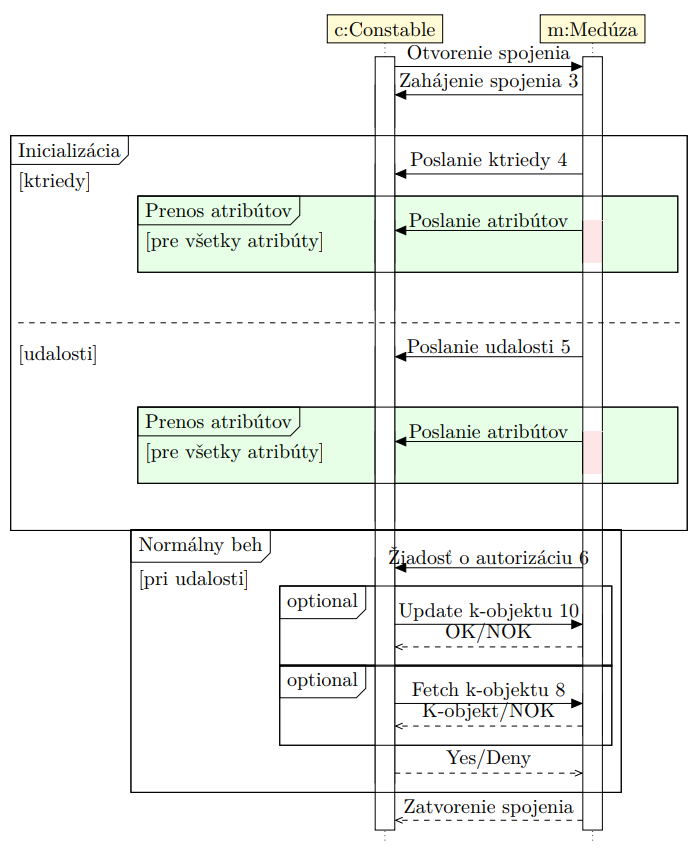
\includegraphics[width=12cm]{img/komunikacia.png}
  \caption{Schéma komunikačného protokolu\cite{kacer}}
  \label{medusakomunikacia}
\end{figure}

\section{Implementácia}
V predchádzajúcich kapitolách sme si popísali entity(štruktúry, funkcie), ktoré je potrebné implementovať v prípade, že chceme rozšíriť bezpečnostné riešenie o ďalší \acrshort{lsm} \textit{hook}. Prvým krokom bolo zadefinovať si \acrshort{lsm} \textit{hook}, ktoré chceme implementovať. Vybrali sme si \acrshort{ipc} mechanizmy semafor, zdieľanú pamäť a fronty správ, ktoré zdieľajú podobnú logiku a ich štruktúry v jadre majú taktiež podobnú kostru. K týmto \acrshort{ipc} mechanizmom prislúchajú \acrshort{lsm} funkcie, ktoré vidíme na ukážke kódu \ref{lst:hook}. 
\subsection{Bezpečnostná štruktúra} \label{securitys}
Ďalším krokom bolo vytvorenie bezpečnostnej štruktúry, ktorá sa ukladá do položky \texttt{security\_s}, ktorá sa nachádza v štruktúre \texttt{kern\_ipc\_perm}, ktorú sme si popísali v kapitole \ref{kernipcperm}. Nami vytvorenú bezpečnostnú štruktúru môžeme vidieť na ukážke štruktúry \ref{lst:securitys} a  jej definícia sa nachádza v súbore \url{include/linux/medusa/l1/ipc.h}. Táto štruktúra obsahuje položku \texttt{ipc\_class}, ktorá definuje o aký typ \acrshort{ipc} mechanizmu ide. Táto položka môže nadobúdať hodnoty 0, 1 alebo 2, ktoré sú definované makrami v rovnakom súbore. Taktiež sa v tejto štruktúre definujú makrá \texttt{MEDUSA\_SUBJECT\_VARS} a \texttt{MEDUSA\_OBJECT\_VARS} ako pri \texttt{k-objekte}, ktoré sme si popísali v kapitole \ref{kobjekt}. 
\begin{lstlisting}[
  caption={Bezpečnostná štruktúra Medusy pre IPC},
  label={lst:securitys},
  language=c
]
#define MED_IPC_SEM 0
#define MED_IPC_MSG 1
#define MED_IPC_SHM 2
#define MED_IPC_UNDEFINED 3

struct medusa_l1_ipc_s {
	unsigned int ipc_class;
	MEDUSA_SUBJECT_VARS;
	MEDUSA_OBJECT_VARS;
};
\end{lstlisting} 

Takto zadefinovanú bezpečnostnú štruktúru je potrebné alokovať načo nám slúžia \acrshort{lsm} \textit{hooky} \texttt{*\_alloc\_security} a na uvoľnenie pamäte \texttt{\_free\_security} tieto \textit{hooky} môžeme vidieť v hornej časti výpisu \ref{lst:hook}. Aj keď tieto funkcie majú rôzne parametre, je možné z týchto parametrov získať položku \texttt{kern\_ipc\_perm}, ktorú využívame v pomocnej funkcií \texttt{medusa\_l1\_ipc\_alloc\_security}, ktorej prvý parameter je práve táto štruktúra a druhým parametrom je typ \acrshort{ipc} mechanizmu. Príklad použitie pomocnej funkcie môžete vidieť na ukážke kódu \ref{lst:allocusage}. Avšak táto pomocná funkcia nepokrýva všetky alokácie, nakoľko \acrshort{lsm} framework obsahuje aj funkciu \texttt{msg\_msg\_alloc\_security}, ktorá má argument typu \texttt{msg\_msg}, ktorý neobsahuje štruktúru \texttt{kern\_ipc\_perm} ale bezpečnostná štruktúra sa nachádza priamo v tejto štruktúre teda \texttt{msg\_msg->security}. Na uvoľnenie pamäte je taktiež vytvorená spoločná funkcia, ktorú môžete vidieť na ukážke kódu \ref{lst:free}. Táto funkcia obsluhuje všetky \acrshort{lsm} \textit{hooky} s výnimkou \texttt{medusa\_l1\_msg\_msg\_free\_security}, ktorá má rovnaké obmedzenia, ktoré sme si spomenuli vyššie, ako funkcia na alokovanie.
\begin{lstlisting}[
  caption={Príklad použitia pomocnej funkcie na alokovanie bezpečnostnej štruktúry},
  label={lst:allocusage},
  language=c
]
static int medusa_l1_msg_queue_alloc_security(struct msg_queue *msq)
{
	return medusa_l1_ipc_alloc_security(&msq->q_perm, MED_IPC_MSG);
}
\end{lstlisting} 

\subsection{Vytvorenie \textit{k-objektu}} \label{kobjectimpl}
Pri definovaný \textit{k-objektu} sme narazili na niekoľko obmedzení, ktoré sa vynorili až v neskorších fázach implementácie a preto sa aj definícia \textit{k-objektu} menila v priebehu vývoja. Prvý priamočiary návrh bolo vytvoriť 3 rôzne \textit{k-objekty} pre \acrshort{sem}, \acrshort{shm} a \acrshort{msg}. Toto riešenie však prinášalo so sebou veľké množstvo kódu nakoľko tieto 3 mechanizmy majú dve operácie \texttt{get} a \texttt{ctl}, ktoré pri svojich volaniach vyvolávaj \acrshort{lsm} \textit{hooky}, ktoré majú signatúry, ktoré môžeme vidieť na ukážke kódu \ref{lst:associate}.
\begin{lstlisting}[
  caption={\acrshort{lsm} \textit{hooky} pre operácie \texttt{get} a \texttt{ctl}},
  label={lst:associate},
  language=c
]
//get
int medusa_l1_[msg_queue/shm/sem]_associate(struct [msg_queue/shmid_kernel/sem_array] *obj, int semflg)
//ctl
int medusa_l1_[msg_queue_msg/shm_shm/sem_sem]ctl(struct [msg_queue/shmid_kernel/sem_array] *obj, int cmd)
\end{lstlisting} 
Keby sme pre každý mechanizmus vytvorili samostatný \textit{k-objekt} a chceli vytvoriť \textit{typ prístupu}, pre tieto dve spomínané operácie vyžadovalo by si to v konečnom dôsledku 6 rôznych \textit{typov prístupu}, keďže \textit{typ prístupu} je v kóde spätý s typom \textit{k-objektu} ako môžeme vidieť v kapitole \ref{acctype}. 
Pre tento fakt sme sa rozhodli vytvoriť 4. \textit{k-objekt}, ktorý predstavuje jednotný \textit{k-objekt}, ktorý sa bude využívať pri \textit{typoch prístupu} a teda pre vyššie spomínané operácie budeme definovať len 2 \textit{typy prístupov}. Všeobecný \textit{k-objekt} môžeme vidieť na ukážke kódu \ref{lst:kobjectcommon}. 
\begin{lstlisting}[
  caption={Všeobecný \textit{k-objekt}},
  label={lst:kobjectcommon},
  language=c
]
struct ipc_kobject {	
	unsigned char data[max_simple(max_simple(sizeof(struct ipc_sem_kobject), sizeof(struct ipc_shm_kobject)), sizeof(struct ipc_msg_kobject))];	
	MEDUSA_OBJECT_VARS;
};
\end{lstlisting} 
Tento \textit{k-objekt} obsahuje položku \texttt{data}. Ide o bajtové pole, ktoré má z definície veľkosť najväčšieho z konkrétnych \textit{k-objektov}. Definíciu vyššie spomínaného \textit{k-objektu} ako aj definície konkrétnych \textit{k-objektov} je možné nájsť v hlavičkovom súbore \url{security/medusa/l2/kobject_ipc_common.h}. 

Konkrétne \textit{k-objekty}(pre \acrshort{sem}, \acrshort{shm} a \acrshort{msg}) obsahujú nasledovné položky:
\begin{itemize}
\item \texttt{ipc\_class} - definuje typ mechanizmu
\item \texttt{ipc\_perm} - predstavuje internú štruktúru Medusy, \texttt{medusa\_ipc\_perm}, ktorá je definovaná v \url{include/linux/medusa/l1/ipc.h}. Obsahuje jednoduché položky štruktúry \texttt{kern\_ipc\_perm}, ktorá bola popísaná v kapitol \ref{kernipcperm} a v štruktúre je definovaná pomocou makra \texttt{MEDUSA\_IPC\_VARS}.
\item \texttt{MEDUSA\_OBJECT\_VARS} - makro, ktoré sme si bližšie popísali v kapitole \ref{kobjekt}
\end{itemize}
Konkrétne \textit{k-objekty} môžu obsahovať aj špecifické údaje pre konkrétny mechanizmus, napríklad \textit{k-objekt} \texttt{ipc\_sem\_kobject} obsahuje položku \texttt{sem\_nsems}, v ktoré je uchovaný počet počítadiel v skupine semaforu.
\subsubsection{Konverzné funkcie} \label{converse}
Takto vytvoreným \textit{k-objektom} je potrebné definovať konverzné funkcie medzi štruktúrou jadra, v našom prípade ide o štruktúry \texttt{msg\_queue}, \texttt{sem\_array} a \texttt{shmid\_kernel} na štruktúry Medusy, ktoré sú \texttt{ipc\_msg\_kobject}, \texttt{ipc\_sem\_kobject} a \texttt{ipc\_shm\_kobject}. Avšak medzi \acrshort{lsm} funkciami sa nachádza aj \texttt{ipc\_permission}, ktorej signatúru môžeme vidieť na ukážke kódu \ref{lst:ipcpermission}.
\begin{lstlisting}[
  caption={Signatúra obslužnej funkcie pre \acrshort{lsm} \textit{hook} \texttt{ipc\_permission}},
  label={lst:ipcpermission},
  language=c
]
static int medusa_l1_ipc_permission(struct kern_ipc_perm *ipcp, short flag)
\end{lstlisting}
Ako môžeme vidieť táto funkcia obsahuje argument \texttt{kern\_ipc\_perm}, ktorý nepredstavuje konkrétnu štruktúru nejakého z mechanizmov ale ide len o podštruktúru. Na základe tohto faktu sme sa preto rozhodli pri konverzných funkciách na vstupe pracovať z touto štruktúrou a zabezpečiť tým kompatibilitu aj pre tento špecificky \acrshort{lsm} \textit{hook}. \textit{K-objekty} pre \acrshort{sem}, \acrshort{shm} a \acrshort{msg} obsahujú vlastné konverzné funkcie v súbore \textit{k-objektu}, teda pre semafor sa nachádzajú tieto funkcie v súbore \url{security/medusa/l2/kobject_ipc_sem.c}. Tieto funkcie majú nasledovné názvy:
\begin{itemize}
\item \texttt{ipc\_[typ]\_kern2kobj} - konverzná funkcia zo štruktúry jadra na štruktúru Medusy
\item \texttt{ipc\_[typ]\_kobj2kern} - konverzná funkcia zo štruktúry Medusy na štruktúru jadra
\end{itemize}
Pričom \texttt{[typ]} môže byť \texttt{sem}, \texttt{shm} alebo \texttt{msg}. Tieto funkcie sa pre každý mechanizmus líšia hlavne v položkách, ktoré sa kopírujú preto si princíp ukážeme len na semaforoch. Na ukážke kódu \ref{lst:ipcsemkern2kobj} môžeme vidieť konkrétnu implementáciu. 
\lstdefinestyle{nm}{basicstyle=\scriptsize\ttfamily,numbers=left,stepnumber=1}
\begin{lstlisting}[
  caption={Konverzná funkcia zo štruktúry jadra na štruktúru Medusy pre \acrshort{sem}},
  label={lst:ipcsemkern2kobj},
  language=c,
  style=nm
]
static struct ipc_sem_kobject storage;

void * ipc_sem_kern2kobj(struct kern_ipc_perm * ipcp)
{
	struct medusa_l1_ipc_s* security_s;
	struct sem_array * sem_array;

	security_s = (struct medusa_l1_ipc_s*) ipcp->security;
	sem_array = container_of(ipcp, struct sem_array, sem_perm);
	
	memset(&storage, '\0', sizeof(struct ipc_sem_kobject));
	
	if(!security_s)
		return NULL;
	
	storage.ipc_class = security_s->ipc_class;
	storage.sem_nsems = sem_array->sem_nsems;
	
	COPY_WRITE_IPC_VARS(&(storage.ipc_perm), ipcp);
	COPY_READ_IPC_VARS(&(storage.ipc_perm), ipcp);
	COPY_MEDUSA_OBJECT_VARS(&storage, security_s);
	return (void *)&storage;
}
\end{lstlisting}

Na začiatku si deklarujeme pomocné premenné, ktoré následne inicializujeme. Prvou pomocnou premennou je bezpečnostná štruktúra, ktorú sme si popísali v kapitole \ref{securitys} a druhou premennou je štruktúra, ktorá je hlavnou štruktúrou pre konkrétny \acrshort{ipc} mechanizmus. Dôležitým makrom, ktoré sa tu používa je makro \texttt{container\_of}. Toto makro na základe ukazovateľa \texttt{ptr} na nejakú položku \texttt{member} dokáže vrátiť adresu na kontajner, ktorý má typ \texttt{type}. Princíp fungovania môžme vidieť aj na obrázku \ref{containerof}.
\begin{figure}[!htbp]
  \centering
  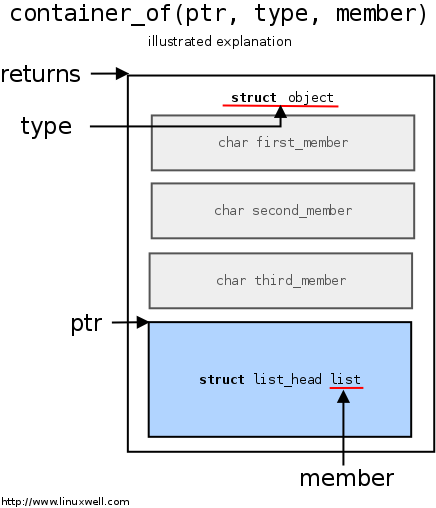
\includegraphics[width=5cm]{img/container_of.png}
  \caption{Princíp fungovania \textit{container\_of} makra \cite{containerof}}
  \label{containerof}
\end{figure}
Pomocou tohto makra dokážeme získať hlavnú štruktúru \acrshort{ipc} mechanizmu len za pomoci štruktúry \texttt{kern\_ipc\_perm}. Ďalším krokom je vynulovanie pamäte premennej \texttt{storage}. Táto premenná slúži na uloženie \textit{k-objektu} v pamäti, pokým sa nepošle autorizačnému serveru. Na ďalšom riadku sa nachádza kontrola bezpečnostnej štruktúry, ktorá by nemala byť \texttt{NULL}, ak však takýto prípad nastane tak funkcia vráti \texttt{NULL} a vyššie funkcie ktoré túto konverziu používajú musia túto možnosť ďalej ošetriť. Na riadku 16 a 17 sa do \textit{k-objektu} prenesú údaje o type mechanizmu a špecifická vlastnosť \acrshort{sem}, ktorou je počet semaforov. Na riadkoch 19 a 20 sú použité pomocné makrá, ktoré sme si vytvorili len pre potreby \acrshort{ipc} a slúžia na prekopírovanie položiek štruktúry \texttt{kern\_ipc\_perm}, ktoré sa v \textit{k-objekte} nachádzajú v položke \texttt{ipc\_perm}, ktorú sme si popísali vyššie v tejto kapitole. Implementácia týchto dvoch makier sa nachádza v hlavičkovom súbore \url{include/linux/medusa/l1/ipc.h}. Makro \texttt{COPY\_READ\_IPC\_VARS} kopíruje položky, ktoré je možné len čítať a makro \texttt{COPY\_WRITE\_IPC\_VARS} kopíruje položky, ktoré je možné čítať aj prepisovať v štruktúre jadra. Posledným makrom, ktoré sa pri konverzii používa je makro \texttt{COPY\_MEDUSA\_OBJECT\_VARS}, ktoré kopíruje interné položky definované pre \textit{objekt} z bezpečnostnej štruktúry do \textit{k-objektu}. Návratová hodnota tejto funkcie je \texttt{void} ukazovateľ na úložisko kde máme nový \textit{k-objekt}.

\begin{lstlisting}[
  caption={Konverzná funkcia zo štruktúry Medusy na štruktúru jadra pre \acrshort{sem}},
  label={lst:ipckobj2kern},
  language=c
]
medusa_answer_t ipc_sem_kobj2kern(struct medusa_kobject_s * ipck, struct kern_ipc_perm * ipcp)
{
	struct medusa_l1_ipc_s* security_s;
	struct ipc_sem_kobject * ipck_sem;

	ipck_sem = (struct ipc_sem_kobject *)ipck;
	security_s = (struct medusa_l1_ipc_s*) ipcp->security;

	COPY_WRITE_IPC_VARS(ipcp, &ipck_sem->ipc_perm);
	COPY_MEDUSA_OBJECT_VARS(security_s, ipck_sem);
	MED_MAGIC_VALIDATE(security_s);
	return MED_OK;
}
\end{lstlisting}

Na ukážke kódu \ref{lst:ipckobj2kern} môžeme vidieť funkciu s opačnou funkcionalitou a teda konverziu z \textit{k-objektu} na štruktúru jadra. Prí takejto konverzii je potrebné si uvedomiť, ktoré položky štruktúry je možné v jadre systému upravovať. Pri \acrshort{ipc} mechanizmoch sme sa inšpirovali operáciou \textit{ctl}, ktorá taktiež má schopnosť meniť štruktúru jadra a práve táto operácie dokáže priamo aktualizovať nasledovné položky \texttt{uid}, \texttt{gid} a \texttt{mode}. Preto aj táto konverzná funkcia môže meniť len tieto tri položky a nemôže meniť napríklad pri semaforoch položku \texttt{sem\_nsems}, čo by mohlo spôsobiť nedefinované správanie. Na zmenu údajov v jadre používame vyššie spomínané makrá pričom na konci vykonávanie funkcie je použité makro \texttt{MED\_MAGIC\_VALIDATE}, ktorého úlohou je nastaviť internú položku Medusy, ktorá indikuje že objekt je už zaregistrovaný v autorizačnom servery. Návratovou hodnotou tejto funkcie je status \texttt{MED\_OK}, ktorý indikuje úspešnú aktualizáciu.

Tieto konverzné funkcie pre \acrshort{sem}, \acrshort{shm} a \acrshort{msg} nie je možné priamo použiť v \textit{type prístupu}, nakoľko ako sme písali v kapitole \ref{kobjectimpl} vytvorili sme 4. všeobecný \textit{k-objekt}. Kvôli tomuto faktu je vytvorená funkcia \texttt{ipc\_kern2kobj}, ktorú môžeme vidieť na ukážke kódu \ref{lst:ipckern2kobj}. Táto funkcia na základe typu \acrshort{ipc} mechanizmu, ktorý získa z  bezpečnostnej štruktúry, rozhodne ktorú konkrétnu funkciu zavolať. Následne skopíruje pamäťovú oblasť kde je uložený \textit{k-objekt} do položky \texttt{data} štruktúry \texttt{ipc\_kobject}. Návratová hodnota funkcie je 0 v prípade úspešnej konverzie v opačnom prípade -1.
\begin{lstlisting}[
  caption={Konverzná funkcia zo štruktúry Medusy na štruktúru jadra},
  label={lst:ipckern2kobj},
  language=c
]
int ipc_kern2kobj(struct ipc_kobject * ipck, struct kern_ipc_perm * ipcp)
{
	struct medusa_l1_ipc_s* security_s;
	unsigned int ipc_class;

	security_s = ipc_security(ipcp);
	ipc_class = security_s->ipc_class;
	switch(ipc_class){
		case MED_IPC_SEM: {
			struct ipc_sem_kobject *new_kobj;
			new_kobj = (struct ipc_sem_kobject *)ipc_sem_kern2kobj(ipcp);
			memcpy(ipck->data, (unsigned char *)new_kobj, sizeof(struct ipc_sem_kobject));
			break;
		}
		...
		default:
			printk("Unkown ipc_class\n");
			return -1;		
	}
	return 0;
}
\end{lstlisting}
\subsubsection{Operácie \textit{fetch} a \textit{update}} \label{ops}
Pre plnohodnotnú funkcionalitu bolo potrebné definovať operácie \textit{fetch} a \textit{update}, ktoré sme si vysvetlili v kapitole \ref{kobjekt}. Tieto operácie sa definujú \textit{k-objektom} konkrétnych mechanizmov, pričom všeobecný \textit{k-objekt}(\texttt{ipc\_kobject}) tieto operácie nedefinuje čo treba zohľadniť pri konfigurácii autorizačného servera. 
\begin{lstlisting}[
  caption={Operácie \texttt{fetch} pre \textit{k-objekt} semaforu},
  label={lst:semfetch},
  language=c
]
static struct medusa_kobject_s * ipc_sem_fetch(struct medusa_kobject_s * kobj)
{
	struct ipc_sem_kobject * ipc_kobj;
	struct medusa_kobject_s * new_kobj;
	ipc_kobj = (struct ipc_sem_kobject *)kobj;
	new_kobj = (struct medusa_kobject_s *)ipc_fetch(ipc_kobj->ipc_perm.id, ipc_kobj->ipc_class, ipc_sem_kern2kobj);
	return new_kobj;
}
\end{lstlisting}
Na ukážke kódu \ref{lst:semfetch} vidíme operáciu \texttt{fetch} \textit{k-objektu} semaforu, ktorá v svojom tele volá funkciu \texttt{ipc\_fetch}. Funkcia \texttt{ipc\_fetch} je spoločná pre všetky 3 \acrshort{ipc} \textit{k-objekty} a jej kód môžeme vidieť na ukážke kódu \ref{lst:fetch}. V tejto spoločnej funkcii sa vykonávajú nasledovné operácie:
\begin{itemize}
\item získanie štruktúry \texttt{ipc\_ids} podľa typu \acrshort{ipc} mechanizmu
\item získanie štruktúry \texttt{kern\_ipc\_perm} na základe identifikátora \acrshort{ipc} mechanizmu
\item konverzia štruktúr pomocou funkcii, ktoré sme si popísali v kapitole \ref{converse}
\item vrátenie nového \textit{k-objektu}
\end{itemize}
\begin{lstlisting}[
  caption={Operácie \texttt{update} pre \textit{k-objekt} semaforu},
  label={lst:semupdate},
  language=c
]
static medusa_answer_t ipc_sem_update(struct medusa_kobject_s * kobj)
{
	struct ipc_sem_kobject * ipc_kobj;
	medusa_answer_t answer;
	ipc_kobj = (struct ipc_sem_kobject *)kobj;
	answer = ipc_update(ipc_kobj->ipc_perm.id, ipc_kobj->ipc_class, kobj, ipc_sem_kobj2kern);
	return answer;
}
\end{lstlisting}
Operácia \textit{update} funguje na rovnakom princípe ale odlišuje sa hlavne v uzamykacích mechanizmoch, ktoré sme tu museli použiť, nakoľko narozdiel od operácie \textit{fetch}, táto operácie mení dáta v štruktúrach jadra a preto je potrebné pomocou rôznych zámkov zabezpečiť zachovanie integrity údajov. Funkciu \texttt{ipc\_update} môžeme vidieť na ukážke kódu \ref{lst:update} a jej použitie na ukážke kódu \ref{lst:semupdate}. Pri \acrshort{ipc} je možné použiť niekoľko druhou zámkou avšak operácie ktoré pod týmito známkami vykonávame sú presne definované a sú nasledovné
\begin{itemize}
\item \texttt{rcu\_read\_lock}/\texttt{rcu\_read\_unlock}
\begin{itemize}
\item počiatočné kontroly (povolenia, audity, ...)
\item len čítacie operácie, ktoré nevyžadujú atomicitu 
\end{itemize}
\item \texttt{ipc\_lock\_object}/\texttt{ipc\_unlock\_object}
\begin{itemize}
\item čítacie operácie, ktoré vyžadujú atomicitu 
\item aktualizácie údajov, ako napríklad \texttt{SET}, \texttt{RMID} príkazy a operácie špecifické pre mechanizmy
\end{itemize}
\item \texttt{ids->rwsem}
\begin{itemize}
\item vytváranie, odstraňovanie a iterácia cez existujúce objekty v \acrshort{ipc} skupine
\item iterovanie cez súbory na ceste \url{/proc/sysvipc/}
\end{itemize}
\end{itemize}
Jadro systému Linux taktiež obsahuje aj operácie na zvýšenie(\texttt{ipc\_rcu\_getref}) a na zníženie(\texttt{ipc\_put\_getref}) počítadla referencii, ktoré zabraňuje tomu aby bol \acrshort{ipc} objekt odstránený a zároveň používaný nejakým procesom. Na základe týchto poznatkov sme v operácii \textit{fetch} použili len \acrshort{rcu} uzamykací mechanizmus keďže vykonávame len čítacie operácie a pri operácií \textit{update} používame systém \acrshort{rcu} spoločne s funkciou \texttt{ipc\_lock\_object} nakoľko vykonávame aj zapisovanie do štruktúr jadra. Aby sme predišli nechcenému odstráneniu objektu zo systému, tak po získaní štruktúry taktiež zvyšujeme aj referenciu na tento objekt. Keďže pri operácii \textit{update} nevytvárame, nemažeme ani neprechádzame objekty \acrshort{ipc}, nebolo potrebné použiť zámok \texttt{ids->rwsem}.
\subsection{Typy prístupov}
Po tom ako sme si vytvorili potrebné \textit{k-objekty}, bolo potrebné zadefinovať \textit{typy prístupov}. Definícia \textit{typu prístupu} priamo nadväzuje na \acrshort{lsm} \textit{hook} avšak snažili sme sa \acrshort{lsm} \textit{hooky}, ktoré sú podobné zlúčiť pod jeden \textit{typ prístupu}. Výsledkom sú nasledovné \textit{typy prístupov}:
\begin{itemize}
\item \texttt{ipc\_ctl} - združuje \textit{hooky} pre operáciu \texttt{ctl}
\item \texttt{ipc\_associate} - združuje \textit{hooky} pre operáciu \texttt{get}
\item \texttt{ipc\_msgrcv}
\item \texttt{ipc\_msgsnd}
\item \texttt{ipc\_permission}
\item \texttt{ipc\_semop}
\item \texttt{ipc\_shmat}
\end{itemize} 
Každý z týchto \textit{typov prístupu} má definovaný \textit{object}, ktorým je aktuálny proces, ktorý získavame pomocou makra \texttt{current} a \textit{subjektom} je \acrshort{ipc} entita, ktorá je typu \texttt{ipc\_kobject}. Taktiež každý \textit{typ prístupu} obsahuje extra položku \texttt{ipc\_class} aby bolo možné na strane autorizačného servera skonvertovať všeobecný \textit{k-objekt} na konkrétny \textit{k-objekt}. Rozdielom medzi týmito \textit{typmi prístupov} sú extra dáta, ktoré sa pridávajú k \textit{typu prístupu}, napríklad pre \texttt{ipc\_semop} sú to položky \texttt{sem\_op}, \texttt{sem\_num}, \texttt{sem\_flg}, \texttt{alter}, ktoré definujú ako a nad čím sa má operácia vykonať. Pre jednotlivé \textit{typy prístupov} je možné tieto položky nájsť v definícii štruktúry \textit{typu prístupu} na začiatku súboru, ako môžeme vidieť na ukážke kódu \ref{lst:acctype}. Ďalej sa v tomto súbore nachádza hlavná funkcia, ktorá na začiatku validuje \textit{k-objekt} procesu ako aj \acrshort{ipc} \textit{k-objekt}, nasleduje kontrola virtuálnych svetov, konverzia dátových štruktúr a na koniec rozhodovanie v podobe volania makra \texttt{MED\_DECIDE}. Ostatné \textit{typy prístupov} môžeme nájsť v priečinku \url{security/medusa/l2/} a súboroch \texttt{acctype\_ipc\_*.c}. 

Aby bolo možné kompletne implementovať \textit{typy prístupov} bolo nevyhnutné vytvoriť \textit{udalosť}, ktorá bude kontrolovať a validovať \textit{k-objekty}. Preto sme vytvorili \textit{udalosť} \texttt{getipc}, ktorá má za úlohu inicializovať interné položky a zaregistrovať objekt u autorizačného serveru. Takto zaregistrovaný objekt považujeme za validný a \textit{typ prístupu} môže ďalej vykonávať rozhodovanie. \textit{Typ prístupu} vyvoláva túto \textit{udalosť} pomocou volania funkcie \texttt{medusa\_ipc\_validate}, ktorej návratová hodnota je typu \texttt{medusa\_answer\_t} a v prípade že nadobúda hodnotu \texttt{MED\_OK} tak rozhodovanie pokračuje v opačnom prípade rozhodovanie nenastane a systému je vrátená hodnota, ktorá povoľuje systémové volanie. Ide o vlastnosť Medusy, ktorá v prípade chyby väčšinou systémové volanie povolí.

Pri implementácii \textit{typov prístupu} sme narazili na problém pri systémovom volaní typu \texttt{ctl}, ktoré sme si popísali aj v kapitole \ref{msguse}. Toto systémové volanie môže byť použité s rôznymi prepínačmi a pri použití prepínača \texttt{IPC\_INFO} alebo \texttt{[type]\_INFO}, kde \textit{type} predstavuje konkrétny \acrshort{ipc}, nastáva situácia kedy do funkcie nevstupuje žiadny \acrshort{ipc} objekt. Preto bolo nevyhnutné tento prípad pri \textit{type prístupu} riešiť a v prípade že sa jedná o jeden zo spomínaných prepínačov tak sa pri rozhodovaní ako objekt posiela \texttt{NULL} a položka \texttt{ipc\_class} v \textit{type prístupu} nadobúda hodnotu \texttt{MED\_IPC\_UNDEFINED}. Toto je potrebné zohľadniť pri konfigurácií aby sa predišlo chybám spôsobením hodnotou \texttt{NULL}. Môže vystávať otázka či je nevyhnutné rozhodovať o systémovom volaní \texttt{ctl} pri takomto použití, teda keď používateľ zisťuje limity \acrshort{ipc} mechanizmu. Avšak z pohľadu útočníka aj toto systémové volanie môže predstavovať vhodný bod na získanie cenných informácií o systéme, ktorý sa snaží skompromitovať a preto je nevyhnutné aj toto volanie kontrolovať.

Takto definované \textit{typy prístupov} sme následne využili vo vrstve L1, kde sme v jednotlivých \acrshort{lsm} \textit{hookoch} zavolali príslušné funkcie. Príklad použitia \textit{typu prístupu} môžeme vidieť na ukážke kódu \ref{lst:l1acctype}.
\begin{lstlisting}[
  caption={Volanie funkcie \textit{typu prístupu} z vrstvy L1},
  label={lst:l1acctype},
  language=c
]
static int medusa_l1_msg_queue_associate(struct msg_queue *msq, int msqflg)
{
	if(medusa_ipc_associate(&msq->q_perm, msqflg) == MED_NO)
		return -EPERM;	
	return 0;
}
\end{lstlisting}

\subsection{Konfigurácia autorizačného servera}
Po doplnení Medusy o ďalšie \textit{typy prístupov} bolo potrebné vytvoriť aj konfiguráciu na strane autorizačného servera s ktorou by sme mohli vykonať testy a odskúšať funkčnosť. Pri našom testovaní sme použili autorizačný server \textit{mYstable} a jeho konfiguráciu v jazyku Python, ktorú môžete vidieť na ukážke kódu \ref{lst:config}. Tento konfiguračný súbor obsahuje pomocnú funkciu \texttt{get\_concrete\_ipc}, ktorej úlohou je na strane autorizačného servera, zmeniť všeobecný \textit{k-object} na konkrétny na základe typu mechanizmu, ktorý sa nachádza v každom \textit{type prístupu} v položke \texttt{ipc\_class}. Ďalej sa v tejto konfigurácii nachádza obsluha pre \textit{udalosť} \texttt{ipc}, ktorá pre jednoduchosť akceptuje všetky požiadavky. Poslednou časťou je samotná obsluha konkrétneho \textit{typu prístupu} a na tejto ukážke je zobrazená obsluha pre \textit{typ prístupu} \texttt{ipc\_ctl}, ktorý sme si taktiež popísali v predchádzajúcej kapitole. Tento \textit{typ prístupu} musí ošetrovať aj prípad kedy typ mechanizmu je 3(\texttt{MED\_IPC\_UNDEFINED}) a v tomto prípade vieme, že ide o špeciálny prípad s príznakom \texttt{IPC\_INFO}, ktorý sme spomínali taktiež v predchádzajúcej kapitole. 

Takto definovaný konfiguračný súbor spolu s ostatnými \textit{typmi prístupov} sme následne použili na kontrolu správnej funkčnosti systému Medusa. Hlavným zdrojom kontroly v našom prípade bol výstup s programu \texttt{dmesg}. Tento program má za úlohu zobraziť zásobník správ jadra a je možné do tohto zásobníka zapisovať pomocou funkcie jazyka C \texttt{printk}. Pre testovacie a ladiace potreby preto Medusa obsahuje špeciálny \textit{k-objekt} \texttt{printk}, ktorý umožňuje na strane autorizačného servera vyvolať operáciu \texttt{update} a zapísať tak do tohto zásobníka v jadre. Pre účeli testovania sme si vytvorili jednoduché programy v jazyku C, ktoré vytvorili \acrshort{ipc} mechanizmy a nakonfigurovali autorizačný server tak aby pomocou \textit{k-objektu} \texttt{printk} zapísal kľúčové informácie o \texttt{ipc} \textit{k-objekte}. Takto sme mohli pozorovať čí sa vo výpise programu \textit{dmesg} po spustení testovacieho programu vypisujú očakávané hodnoty a overiť správnu funkčnosť systému Medusa.
